\chapter{Модель картины мира. Синтаксический уровень} \label{chapt2}

По представлениям психологов \cite{Chudova2012,Chudova2014} когнитивные функции субъекта, носителя картины мира, работают в двух <<режимах>>: биологическом и культурном. В первом режиме базовой отправной точкой работы психики является сигнал "--- абиотический стимул, используемый субъектом как указатель на определённый биотический стимул, при этом психические функции работают на распознавание биологически значимой ситуации удовлетворения некоторой потребности (физиологической или социальной). Во втором режиме определяющую роль играет знак "--- материальный объект, его свойство или некоторое явление, используемые субъектом как указатель на смысл события, т.\,.е. на собственное желание или желание другого. Знак в этом случае связывает природное и культурное явления, а психические функции работают над задачей понимания сообщения. В данной главе будет рассмотрен внешний, синтаксический уровень модели картины мира, в которой когнитивные функции выполняются именно в знаковом, культурном <<режиме>>.

\section{Знак"--~базовый элемент картины мира} \label{sect2_1}

По А.\,Н.~Леонтьеву \cite{Leontiev1975} представление каждого объекта или процесса в картине мира включает три компоненты: \textit{образ} явления, его \textit{значение} и \textit{личностные смыслы} субъекта, связанные с этим явлением. Для краткости далее вместо словосочетания представление каждого явления в картине мира будет использоваться словосочетание элемент картины мира.

Образ явления представляет собой процедуру обнаружения и отделения этого явления от других, которая реализуется либо низкоуровневыми физиологическими механизмами восприятия, либо высокоуровневыми действиями, требующими специального предварительного акта планирования. Значение представляет собой выработанные в рамках культурно-исторического процесса коллективом, которому принадлежит данный субъект, общепринятые способы использования данного явления в деятельности субъекта, в том числе наборы ситуаций с участием данного явления, в которых принято совершать определённые действия. Наконец, личностный смысл определяет отношение данного явления к той или иной потребности субъекта, которая может быть удовлетворена с помощью набора действий, определяемым самим субъектом на основе своего опыта.

Образ потенциального элемента картины мира, его значение и смыслы могут не связываться в единое целое, и тогда не происходит формирования (в филогенезе) или актуализации (в микрогенезе) знака. В таком случае психическое отражение фиксирует для субъекта не личностный, а \textit{биологический смысл} объекта, не образ мышления, но образ восприятия (\textit{перцепт}), и \textit{функциональное значение} объекта в решаемой задаче вместо значения, выработанного в ходе общественно-исторической практики. Такое внезнаковое отражение реальности позволяет осуществлять лишь <<парные>> переходы между двумя компонентами знания о явлении: 
\begin{itemize}
	\item от перцепта к функциональному значению "--- выбор способа использования конкретного объекта, 
	\item от функционального значения к биологическому смыслу "--- выбор <<цели>> для конкретного действия, 
	\item от биологического смысла к перцепту "--- выбор конкретного объекта, удовлетворяющего заданным критериям.
\end{itemize}
Поскольку три аспекта знания об объекте связаны в этом случае лишь парными зависимостями, то нужен <<внешний наблюдатель>>, чтобы увидеть, что это три компоненты отражения одного явления реального мира \cite{Chudova2012}.

До момента связывания в знак три компоненты будем называть перцептом, биологическим смыслом и функциональным значением соответственно. Связывание упомянутых трёх компонент в единую структуру позволяет перейти к рассмотрению явления как целостного и существующего независимо от текущего состояния действующего субъекта. Такое связывание становится возможным благодаря именованию возникающей структуры, что приводит к конструкции, называемой \textit{знаком}. При этом знак и его компоненты становятся элементами \textit{языковой системы}, т.\,е. осуществляется включение знака в картину мира субъекта (чего не происходит без именования). Сам объект приобретает при этом устойчивое и общепринятое значение, личный опыт действования с ним отражается в личностном смысле как компоненте знака, а событие восприятия объекта, представляющее собой в простейшем случае отражение в симультанном <<рисунке>> процедуры воспроизведения свойств объекта моторикой воспринимающего органа, фиксируется как образ явления.

%\newpage
%============================================================================================================================

\section{Процесс формирование нового знака} \label{sect2_2}

Следуя \cite{PanovA2014a} приведём схему процесса формирования (актуализации) знака.
\begin{enumerate}
	\setcounter{enumi}{-1}
	\renewcommand\labelenumi{\theenumi.}
	\item\label{step0} Локализация явления. Происходит это в пространстве, в котором наряду с четырьмя измерениями физического пространства"--~времени существует пятое квази"--~измерение "--- измерение значений \cite{Leontiev1983}. При этом субъект определяет положение явления относительно самого себя. Это значит, что он должен реализовывать функцию самосознания (рефлексию), знать свои <<координаты>> в этом пространстве, т.\,е. пребывать, как говорят психиатры, в состоянии ясного сознания (уметь определить не только физические, но и социальные параметры самого себя и ситуации, в которой он оказался).
	\item\label{step1} Формирование перцепта. Основано на работе процедуры воспроизведения свойств явления моторикой воспринимающего органа (для живых существ) или на обработке методами распознавания образов информации, снимаемой с датчиков (для искусственных систем).
	\item\label{step2} Порождение на основе прошлого опыта или на основе прецедентов в виде множества пар <<перцепт "--- функциональное значение>> и сформированного на шаге \ref{step1} перцепта "--- функционального значения явления.
	\item\label{step3} Оценка специальным механизмом степени близости функционального значения, полученного на стадии \ref{step2} к функциональному значению, полученному на стадии \ref{step0}; в случае недостаточной близости "--- переход к шагу \ref{step1} и продолжение формирования перцепта (в психологии сенсорно"--~перцептивных процессов этот механизм получил название <<сенсорная уверенность>>).
	\item\label{step4} Стадии \ref{step1}--\ref{step3} выполняются до получения степени близости, достаточной с точки зрения специального механизма, упомянутого на шаге \ref{step3}.
	\item\label{step5} Получение субъектом из культурной среды, аккумулированной в системе естественного языка, пары <<имя знака "--- значение>> и оценка специальным механизмом степени близости функционального значения, построенного на стадии \ref{step4} к значению, полученному из культурной среды; в случае недостаточной близости "--- переход к шагу \ref{step1} и продолжение формирования перцепта.
	\item\label{step6} Связывание имени из пары <<имя знака "--- значение>> с перцептом, построенным после завершения выполнения шагов \ref{step1}--\ref{step5}. С этого момента перцепт превращается в образ.
	\item Формирование личностных смыслов знака на основе прецедентов действий с явлением.
	\item Связывание имени из пары <<имя знака "--- значение>> со сформированным личностным смыслом. С этого момента функциональное значение превращается в значение, а биологический смысл "--- в личностный смысл.
	\item Продолжение отображения <<биологический смысл "--- перцепт>> включением в область определения отображения личностного смысла, полученного в предыдущем пункте, а в область значений "--- образа из шага \ref{step6}.
\end{enumerate}

В результате образован знак, соответствующий явлению. При этом следует отметить, что в следствие шага \ref{step2} формирование знака вне культурной среды невозможно. Далее будет дано уточнение приведённой схеме.

\subsection{Компоненты знака и процедуры связывания}\label{subsect2_2_1}

Итак, пусть:
\begin{itemize}
	\item $A$ "--- множество смыслов (как личностных, так и биологических),
	\item $M$ "--- множество значений,
	\item $P$ "--- множество признаков объектов.
\end{itemize}

Тогда:
\begin{itemize}
	\item $a\subseteq A$ "--- подмножество множества личностных смыслов (возможно пустое),
	\item $m\subseteq M$ "--- подмножество множества значений (функциональное либо культурно"--~историческое),
	\item $p\subseteq P$ "--- подмножество множества признаков (перцепт либо образ) (рис. \ref{fg:sign}).
\end{itemize}

\begin{figure}[h]
	\centering
	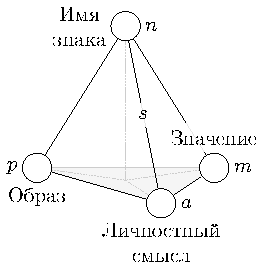
\includegraphics[width=0.5\linewidth]{sign}
	\caption{Знак и его структура.}
	\label{fg:sign}
\end{figure}

Переходы от множества признаков $Р$ к его различным подмножествам реализуются благодаря наличию у субъекта действования встроенных процедур распознавания образов. Процесс формирования знака начинается с работы именно этих процедур. Благодаря им происходит переход от универсального множества свойств $Р$ к его подмножеству, представляющему рассматриваемое явление и отделяющему его от остальных. На первом этапе формирования знака этот процесс приводит к формированию образа восприятия или перцепта. На внутреннем или семантическом уровне построению перцепта соответствует последовательное применение некоторого множества процедур распознавания образов, чему посвящён параграф \ref{sect3_1}.

Что касается значения $m$, то на первом этапе формирования знака подмножества $m$ из $М$ суть функциональные назначения предмета, т.е. способы его использования, далее превращающиеся в значения. Итерационная процедура формирования функционального значения подробно описана в параграфе \ref{sect3_2}.

Подмножество $а$ множества личностных смыслов $А$ возникает благодаря опыту действования с предметом. Всякое подмножество личностных смыслов а будем интерпретировать как множество таких действий с предметом, соответствующим знаку, которые некоторым специальным механизмом оценены как успешные. Этот <<специальный>> механизм есть одна из процедур самосознания и в данной работе подробно не рассматривается. Формирование личностного смысла осуществляется на основе прецедентов.

Введём далее отображения связывания. Заметим, что эти отображения являются частичными функциями из булеанов $P$, $M$ и $А$ в булеаны $М$, $А$ и $Р$ соответственно. Наша цель "--- продемонстрировать, каким образом эти отображения строятся субъектом деятельности. Разумеется, будем полагать, что субъект уже обладает минимальным опытом, т.е. ранее выполнял какие-то действия.

Первое из таких отображений $\Psi_p^m:2^P\rightarrow 2^M$ "--- процедура связывания образа (или перцепта) $p$ с (функциональным) значением $m$ так, что $\Psi_p^m(p^{(i)})=m^{(i)}$, где $p^{(i)}\in 2^P$, $m^{(i)}\in 2^M$, $2^P$ и $2^M$ "--- булеаны $P$ и $M$ соответственно.

Второе отображение $\Psi_m^a:2^M\rightarrow 2^A$ связывает значения (или функциональные значения) с личностными (или биологическими) смыслами таким образом, что $\Psi_m^a(m^{(i)})=a^{(i)}$, где $m^{(i)}\in 2^M$, $a^{(i)}\in 2^A$, $2^A$ "--- булеан $A$. Отображение $\Psi_a^p:2^A\rightarrow 2^P$ связывает личностные (или биологические) смыслы с образом (перцептом) так, что $\Psi_a^p(a^{(i)})=p^{(i+1)}$, где $a^{(i)}\in 2^A$, $p^{(i+1)}\in 2^P$.

Все перечисленные выше процедуры являются итерационными (верхние индексы в скобках соответствуют номеру итерации). Действуя на основе приведённой в начале настоящего параграфа схемы рассмотрим стадии формирования знака предмета в микрогенезе или стадии актуализации знака.

\subsection{Формирование функционального значения и образа восприятия} 

Как было сказано выше, считается, что субъект обладает некоторым опытом действования, который зафиксирован, в частности, в прецедентах (примерах) применения отображения $\Psi_p^m:2^P\rightarrow 2^M$. Будем считать, что множество прецедентов есть множество упорядоченных пар вида $\langle p,m\rangle$ таких, что $\Psi_p^m(p^{(i)})=m^{(i)}$, где $p^{(i)}\in 2^P$, $m^{(i)}\in 2^M$.

Применим для описания процесса формирования перцепта и функционального значения элементарные топологические соображения. Заметим, что $(P, T_P)$ и $(M, T_M)$ суть дискретные топологические пространства с топологиями $T_P=2^P$ и $T_M=2^M$ соответственно. Тогда отображение $\Psi_p^m: 2^P\rightarrow 2^M$ есть отображение топологического пространства $(P, T_P)$ в топологическое пространство $(M, T_M)$. Пусть $N=\langle i_1,i_2,\dots,i_n\rangle$ "--- последовательность итераций отображения $\Psi_p^m$ топологического пространства $(P, T_P)$ в топологическое пространство $(M, T_M)$. Тогда бинарное отношение $\geqslant$ является направлением на $N$, а $(\Psi_p^m | N, \geqslant)$ "--- последовательностью по направленному множеству $N$. Поскольку $\Psi_p^m(p^{(i)})=m^{(i)}$, где $m^{(i)}\in (M,T_M)$, то $\Psi_p^m$  "--- направленность в $М$.

Пусть $m$ "--- некоторая точка в пространстве $(M,T_M)$, $\sigma$ "--- система окрестностей точки $m$. В результате применения отображения $\Psi_m^p$ (т.е. отображения, обратного $\Psi_p^m$) возникает некоторый начальный перцепт $p^{(0)}$.

В результате работы механизмов распознавания образов (рассмотрение которых здесь опущено) в $(P,T_P)$ формируется перцепт $p^{(1)}$. Отображение $\Psi_p^m$ ставит ему в соответствие функциональное значение $m^{(1)}$ из $(M,T_M)$.

Далее возможны три случая:
\begin{enumerate}
	\item\label{choise_1} $m^{(1)}=m$,
	\item\label{choise_2} $m^{(1)}\not\in\sigma$,
	\item\label{choise_3} $m^{(1)}\in\sigma$.
\end{enumerate}

Начнём со случая \ref{choise_2}. Для большей определённости допустим, что $p^{(1)}$ "--- одноэлементное множество. Тогда если $m^{(1)}\not\in\sigma$, то следует выбрать, вообще говоря, другое одноэлементное множество $p^{(2)}$ и вновь применить отображение $\Psi_p^m(p^{(2)})=m^{(2)}$. Содержательно это означает, что признак $p^{(1)}$ был выбран неудачно и не являлся существенным. С точки зрения распознавания образов требуется настройка процедур распознавания. Этот процесс продолжается до тех пор, пока не будет получен случай \ref{choise_3}.

В случае \ref{choise_3} имеет место следующее: тогда и только тогда, когда, начиная с некоторого $k$, последовательность $(\Psi_p^m,\geqslant)$ по направленному множеству $(\Psi_p^m | N,\geqslant)$ остается в окрестности $\sigma$ точки $m$, тогда она сходится к точке $m$. Однако топология $(M,T_M)$ является дискретной, в которой любое множество открыто; тогда из того, что $m$ "--- предел последовательности $(\Psi_p^m,\geqslant)$, следует, что $m^{(i)}=m$, начиная с некоторого $k$. Этим исчерпывается и случай \ref{choise_1}. Следовательно, $p^{(i)}={(\Psi_p^m)}^{-1}(m)=\Psi_m^p(m)$.

Далее в соответствие с приведённой схемой субъект получает из внешней культурно"--~исторической среды пару <<имя "--- значение>> "--- $\langle n,m^0\rangle$. Пусть $\sigma^0$ "--- система окрестностей точки $m^0$ в $(M,T_M)$. Тогда вновь следует рассмотреть три случая:
\begin{enumerate}
	\item\label{choise0_1} $m=m^0$,
	\item\label{choise0_2} $m\not\in\sigma^0$,
	\item\label{choise0_3} $m\in\sigma^0$.
\end{enumerate}

Если $m\not\in\sigma^0$, то необходимо вновь применить процедуры распознавания и отображение $\Psi_p^m$ до тех пор, пока не будет получен случай \ref{choise0_3}. Остаётся только использовать приведённые в предыдущем абзаце соображения, заменив $\sigma$ на $\sigma^0$, а $m$ "--- на $m^0$. Завершается эта стадия монотонным продолжением функции $\Psi_p^m$ на множество $\{\langle p^{(i)},m^0\rangle\}$.

\subsection{Именование}

Будем рассматривать процедуру получения из внешней среды пары $\langle n,m\rangle$ как функцию $\mathfrak M(n)$, выдающую по имени $n$ значение $m$. Тогда ${(\Psi_p^m)}^{-1}(\mathfrak M(n))$ есть функция, присваивающая имя $n$ перцепту $p^\prime$. Обозначим ее через $\mathfrak P(n)$. Иначе говоря, $\mathfrak P(n)$ есть функция именования перцепта. С получением имени $n$ перцепт $p^\prime$ превращается в образ $p$. На следующем шаге выполняется именование биологических смыслов и тем самым "--- трансформация их в личностные смыслы.

Множество личностных смыслов, как было замечено выше, формируется на основе опыта действий субъекта деятельности с предметом, соответствующим рассматриваемому знаку, и оценки успешности этих действий с помощью механизмов самосознания. Для определённости будем полагать, что этот опыт зафиксирован в отображении $a=\Psi_m^a(m)$, т\,.е. в виде пары $\langle m,a\rangle$. Тогда функция $\mathfrak A(n)$ именования биологического смысла $a^\prime$ будет иметь следующий вид: $\mathfrak A(n)=\Psi_m^a(\mathfrak M(n))$. Биологический смысл $a^\prime$ становится личностным смыслом $a$ (рис. \ref{fg:sign_naming}). Завершается этот процесс монотонным продолжением функции $\Psi_a^p$ на множество $\{a\}$.

\begin{figure}[h]
	\centering
	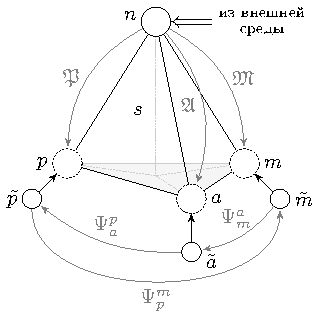
\includegraphics[width=0.5\linewidth]{sign_naming}
	\caption{Процедуры связывания компонент знака и функция именования.}
	\label{fg:sign_naming}
\end{figure}

Легко видеть, что имеют место следующие факты.
\begin{Pred}
	\label{pred:fixed_point}
	Если $s$ "--- знак, $p$, $m$, $a$ "--- его образ, значение и личностный смысл, соответственно, то тройка $\langle p,m,a\rangle$ есть неподвижная точка оператора $\Psi_a^p\Psi_m^a\Psi_p^m$.
\end{Pred}
\begin{Proof}
	Действительно, если $n$ "--- имя знака $s$, то тогда значениями функций именования $\mathfrak P$, $\mathfrak M$ и $\mathfrak A$ в точке $n$ являются соответствующие компоненты знака. В этом случае из определения процедур связывания следует, что $\Psi_p^m(\mathfrak P(n))=\mathfrak M(n)$, $\Psi_m^a(\mathfrak M(n))=\mathfrak A(n)$ и $\Psi_a^p(\mathfrak A(n))=\mathfrak P(n)$. Рассмотрим пространство $Z$, в котором каждая точка $z_i$ представлена тройкой $\langle p_i,m_i,a_i\rangle$. В этом пространстве действие операторов $\Psi_x^y$, $x,y\in\{p,m,a\}$, является поокординатным преобразованием точки, т.е. применение, к примеру, оператора $\Psi_p^m$ к точке $z_i=\langle p_i,m_i,a_i\rangle$ означает преобразование второй координаты таким образом, что в результирующей точке $z'_i=\langle p_i,m'_i,a_i\rangle$ $m'_i=\Psi_p^m(p_i)$. Тогда последовательное покоординатное применение операторов $\Psi_a^p$, $\Psi_m^a$, $\Psi_p^m$ к точке $\langle p,m,a\rangle$, для которой существуют указанные выше функции именования, не приведёт к изменению её координат, т.е. $\Psi_a^p\Psi_m^a\Psi_p^m(\langle p,m,a\rangle)=\langle p,m,a\rangle$, что и требовалось доказать.
\end{Proof}

\begin{Pred}
	Если $s$ "--- знак, то  $\Psi_m^a\Psi_p^m\Psi_a^p$, $\Psi_a^p\Psi_m^a\Psi_p^m$ и $\Psi_p^m\Psi_a^p\Psi_m^a$ "--- тождественные операторы.
\end{Pred}	
\begin{Proof}
	Так как задан знак со своими компонентами, то выполняется условие утверждения \ref{pred:fixed_point} и действие оператора $\Psi_a^p\Psi_m^a\Psi_p^m$ можно записать следующим образом:  $p=\Psi_a^p(a)=\Psi_a^p(\Psi_m^a(m))=\Psi_a^p(\Psi_m^a(\Psi_p^m(p)))$, что и означает тождественность данного оператора. Аналогичным образом выписывается тождественность остальных операторов.
\end{Proof}

\begin{Pred}
	Если $s$ "--- знак, то $\Psi_p^m(\mathfrak P(n))=\mathfrak M(n)$, $\Psi_m^a\Psi_p^m(\mathfrak P(n))=\mathfrak A(n)$.
\end{Pred}	
\begin{Proof}
	Данные тождества следуют из доказательства утверждения \ref{pred:fixed_point}.
\end{Proof}

Подобным образом выписываются ещё шесть фактов такого рода.

%\newpage
%============================================================================================================================

\section{Отношения и процедуры самоорганизации} \label{sect2_3}

Рассмотрим структуры, которые могут возникать на множестве знаков как результат их самоорганизации. Моделирование самоорганизации в картине мира позволяет операционализировать представления об <<активности знаний>> \cite{Osipov2002b}, сформировавшееся в искусственном интеллекте под влиянием предложенной Л.~Фестингером в 1956~г. концепции побуждающей роли знаний в поведении человека. Согласно Л.~Фестингеру, знания не просто накапливаются и используются субъектом "--- знания живут своей жизнью, вступают в отношения, образуют то гармоничные, согласованные системы представлений, то оказываются втянуты в конфликты и противопоставляются друг другу. Последний случай, случай рассогласования в знаниях, и выступает как побуждающая поведение сила: <<\dots взгляды и установки имеют свойство объединяться в систему, характеризующуюся согласованностью входящих в неё элементов \dots существование противоречивых отношений между отдельными элементами в системе знаний, само по себе является мотивирующим фактором>> \cite{Festinger1999}.

\subsection{Отношения и операции на множестве образов}\label{subsect_2_3_1}

Пусть $S=\{s_1,s_2,\dots,s_k\}$ "--- множество знаков, $p=(x_1,x_2,\dots,x_g)$ и $q=(y_1,y_2,\dots,y_h)$ "--- образы знаков $s_p$ и $s_q$ соответственно ($p,q\in(2,\dots,k)$).
Пусть $\pi$ "--- множество образов знаков из $S$. Образы $p$ и $q$ из $\pi$ суть множества значений признаков; индексы признаков указывают на их принадлежность тем или иным множествам признаков (доменам); так равенство $i=j$ свидетельствует о принадлежности значений признаков $x_i$ и $y_j$ одному и тому же множеству, например $X_i$.

Упорядоченные множества $\tau_p=\langle i_1,i_2,\dots,i_p\rangle$ и $\tau_q=\langle j_1,j_2,\dots,j_q\rangle$, где $i_1,i_2,\dots,i_p\in(1,\dots,g)$, $j_1,j_2,\dots,j_q\in(1\dots,h$, будем называть типами образов знаков $s_p$ и $s_q$ соответственно.

Введём оператор $Pat$, который для всякого знака $s_p$, просматривает все остальные знаки и выполняет указанные ниже действия (пополняет бинарные отношения).
\begin{enumerate}
	\renewcommand\labelenumi{\theenumi.}
	\item Если для знака $s_p$ и некоторого знака $s_q$ ($p\not =q$) $\tau_p=\tau_q$ и $x_i=y_i$, то $R_1:=R_1\cup\{(p,q)\}$, $R_1\subseteq\pi\times\pi$.
\end{enumerate}
Легко видеть, что отношение $R_1$ является отношением эквивалентности на множестве образов $\pi$. Определённые ниже отношения $R_2$, $R_3$, $R_4$ есть отношения включения, сходства и противопоставления соответственно.
\begin{enumerate}
	\setcounter{enumi}{1}
	\renewcommand\labelenumi{\theenumi.}
	\item Если для знака $s_p$ и некоторого знака $_q$ $\tau_p\subset\tau_q$ и $\forall i\in\tau_p$ имеет место $x_i=y_i$, то $R_2:=R_2\cup\{(p,q)\}$, $R_2\subseteq\pi\times\pi$ (отношение включения).
	\item Если для знака $s_p$ и некоторого знака $s_q$ $\tau_p\cap\tau_q\not =\varnothing$ и $\forall i\in(\tau_p\cap\tau_q)$ имеет место $x_i=y_i$, то $R_3:=R_3\cup\{(p,q)\}$, $R_3\subseteq\pi\times\pi$ (отношение сходства).
	\item Если для знака $s_p$ и некоторого знака $s_q$ $\tau_p\cap\tau_q\not =\varnothing$ и $\forall i\in(\tau_p\cap\tau_q)$ имеет место $x_i\not =y_i$, то $R_4:=R_4\cup\{(p,q)\}$, $R_4\subseteq\pi\times\pi$ (отношение противопоставления).
\end{enumerate}

По существу, приведённые определения суть процедуры порождения новых элементов отношений на множестве знаков. Стартуя всякий раз, когда множество знаков пополняется новым знаком (или когда множество знаков начинает использоваться), описанные процедуры либо формируют новое отношение, либо пополняют какое-либо из отношений на знаках новым элементом. Это означает, что взаимодействие образов различных знаков приводит к формированию на множестве образов неоднородной семантической сети \cite{Osipov1990} с четырьмя типами отношений: эквивалентность образов, включение образов, сходство образов и противопоставление образов.

Рассмотрим в качестве примера операцию обобщения. Частичная операция обобщения $\Theta$ определена на множестве пар образов, принадлежащих отношению $R_3$; результатом работы $\Theta$ является новый образ, включающий все общие признаки исходных образов. Пусть $\pi$ "--- множество образов, $р_1,р_2\in\pi$, $р_1=(x_1,x_2,\dots,x_g)$ и $р_2=(y_1,y_2,\dots,y_h)$, тогда $\Theta:\pi\times\pi\rightarrow\pi$ так, что для всяких $р_1,р_2\in\pi$ таких, что $(р_1,р_2)\in R_3$, $\Theta(р_1,р_2)=р_3$, где $р_3=(z_1,z_2,\dots,z_l)$ так, что для $\forall j\exists j,k$, такие, что $z_i=x_j=y_k$.

Построенный в результате выполнения операции обобщения образ может послужить основой для формирования нового знака. Новый знак образуется аналогично формированию знака, описанному в разд.2, с некоторыми модификациями.
\begin{enumerate}
	\renewcommand\labelenumi{\theenumi.}
	\item Порождение на основе прошлого опыта или на основе прецедентов множества пар вида <<образ "--- значение>> "--- значения знака.
	\item Получение субъектом из культурной среды, аккумулированной в системе естественного языка, пары <<имя знака "--- значение>>.
	\item Связывание имени из пары <<имя знака "--- значение>> с образом.
	\item Формирование личностных смыслов знака на основе прецедентов действий с предметами, описываемыми обобщённым образом.
	\item Связывание имени из пары <<имя знака "--- значение>> со сформированным личностным смыслом.
	\item Продолжение отображения <<личностный смысл "--- образ>> включением в область определения отображения личностного смысла, полученного в предыдущем пункте, а в область значений "--- образа, построенного в п.1.
\end{enumerate}

В результате образуется знак, соответствующий обобщённому образу. При этом пары образов $(р_3,р_1)$ и $(р_3,р_2)$ пополняют отношение включения $R_2$. Новый знак $s_3$ является для знаков $s_1$ и $s_2$ их обобщением по образам (рис. \ref{fg:pattern_gen}).

\begin{figure}[h]
	\centering
	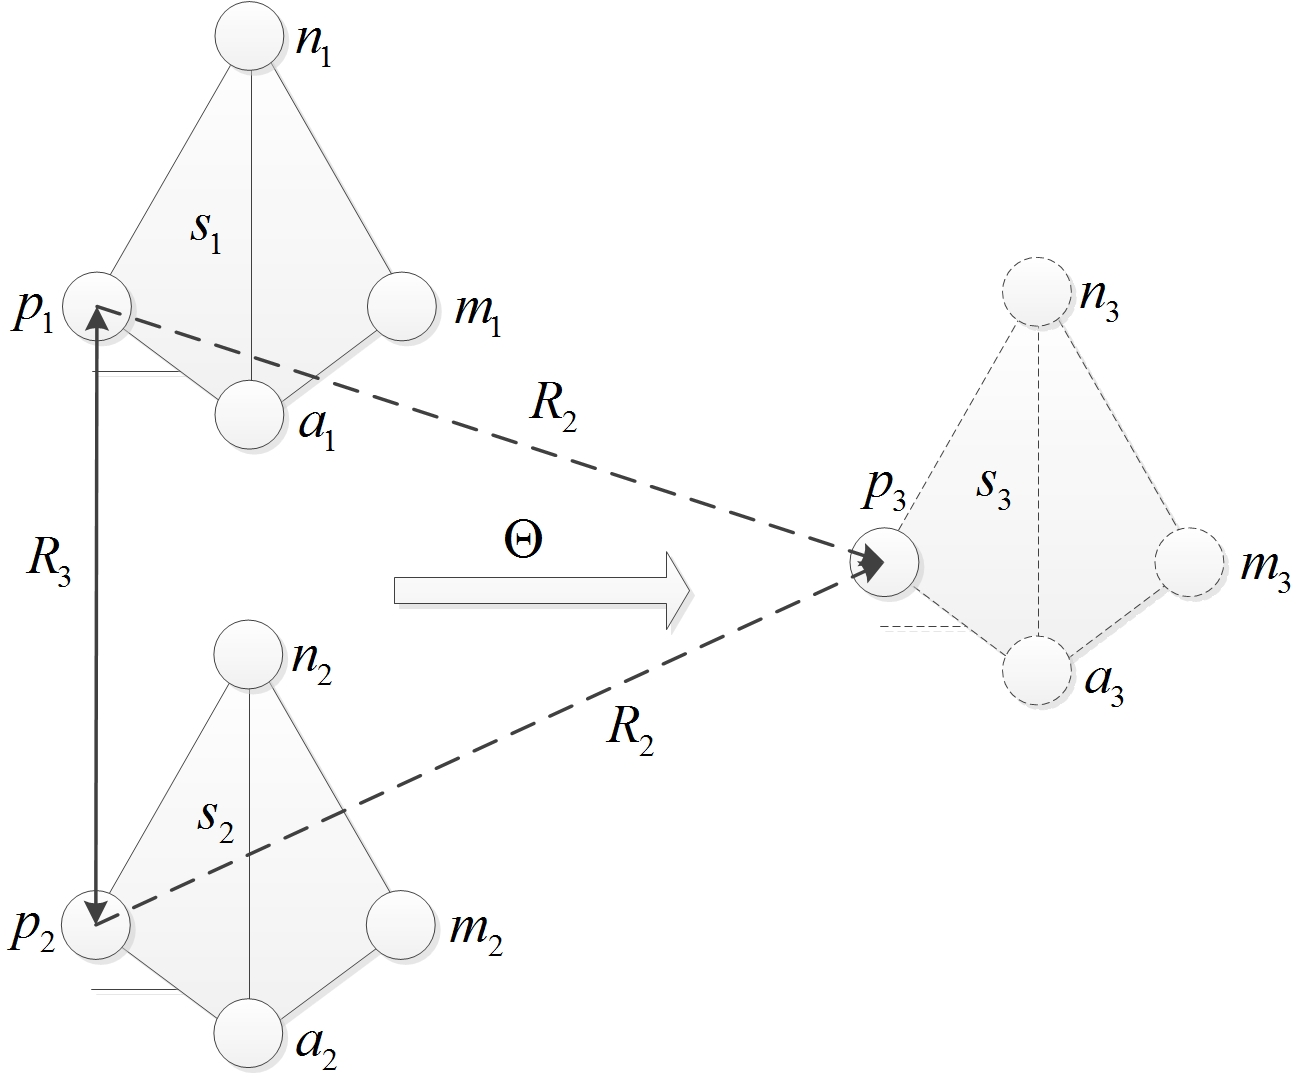
\includegraphics[width=0.7\linewidth]{pattern_gen.jpg}
	\caption{Пример обобщения по признакам. В результате работы операции обобщения $\Theta$ пары знаков $s_1$ и $s_2$, принадлежащих отношению сходства $R_3$, формируется образ $p_3$ нового знака $s_3$ так, что пары $(p_3, p_1)$ и $(p_3, p_2)$ пополняют отношение включения $R_2$.}
	\label{fg:pattern_gen}
\end{figure}

\subsection{Отношения и операции на множестве личностных смыслов}

Как мы видели, с каждым знаком связан некоторый личностный смысл. На множествах личностных смыслов различных знаков оператор $Mean$ естественным образом порождает отношения поглощения, противопоставления и агглютинации (т.е. склеивания, присоединения) смыслов. Определим эти отношения. Пусть по-прежнему $S=\{s_1 s_2,\dots,s_k\}$ "--- множество знаков.

Введём множество действий $ACT$ и функцию $I$, отображающую множество личностных смыслов в булеан $2^{ACT}$ множества действий \cite{Osipov2000}, т.е. функцию, каждому личностному смыслу $a$ из $2^A$ ставящую в соответствие некоторое подмножество $act\in ACT$: $I:2^A\rightarrow 2^{ACT}$ так, что для $\forall а\in 2^A I(а)=act,act\in 2^{ACT}$.

Для всякого знака $s$ отображение $I$ ставит в соответствие каждому личностному смыслу $а$ этого знака множество действий $act$, применимых к объекту, опосредуемому знаком $s$. Эту функцию назовём интерпретацией.

Пусть теперь $I(a_1)=(\alpha_1,\alpha_2,\dots,\alpha_g)$ и $I(a_2)=(\beta_1,\beta_2,\dots,\beta_h)$ "--- интерпретации личностных смыслов знаков $s_1$ и $s_2$. Если действие $\alpha_i$ добавляет некоторый факт \cite{Osipov2000}, а действие $\beta_j$ удаляет тот же факт \cite{Osipov2000}, то будем говорить, что $\alpha_i$ и $\beta_j$ противопоставлены друг другу и принадлежат отношению $R_5:=R_5\cup\{(\alpha_i,\beta_j)\}$, $R5\subseteq AСТ\times AСТ$ "--- отношению оппозиции, т.е. множеству пар действий, образующих оппозиционные шкалы в смысле \cite{Kelly1991}.

Определим следующие отношения на множестве личностных смыслов:
\begin{enumerate}
	\item $\sqsubseteq(a_1,a_2)$ или $a_1\sqsubseteq a_2$ (читается <<смысл $a_2$ поглощает смысл $a_1$>>), если $I(a_1)\subseteq I(a_2)$;
	\item $\perp(a_1,a_2)$  или $a_1\perp a_2$ (<<смысл $a_1$ противопоставлен смыслу $a_2$>>), если $\exists\alpha_1\in a_1,\beta_j\in a_2$, что $(\alpha_i,\beta_j)\in R_5$;
	\item $\sqcup(a_1,a_2,a_3)$ "--- трёхместное отношение агглютинации смыслов, если $I(a_1)\cup I(a_2)=I(a_3)$.
\end{enumerate}

\subsection{Отношения и операции на множестве значений}

Как было сказано выше, значение всякого знака отражает принятые в обществе способы использования соответствующего знаку предмета и поэтому может интерпретироваться некоторым действием. Тогда интерпретация значения напрямую связана с интерпретациями элементов личностного смысла знака. Отметим, что личностный смысл, в отличие от значения, отражает индивидуальные предпочтения субъекта, в то время как значение отражает принятые в обществе способы использования соответствующего знаку предмета. В лексике языка значение, таким образом, может отражаться некоторой группой синонимичных предикатных слов: глаголом, девербативом (т.~е. отглагольным существительным), причастием, деепричастием, которые единственным образом характеризуются своим набором семантических валентностей \cite{Schank1972}.

Пусть $I=\{i_1,i_2,\dots,i_q\}$ "--- множество всех возможных семантических валентностей, тогда каждую группу синонимичных предикатных слов можно характеризовать каким-либо подмножеством этого множества: $I_m=\{j_1,j_2,\dots,j_k\}$, $I_m\subseteq I$. Например, группу предикатных слов движения (<<ехать>>, <<бежать>>, <<идти>>) можно охарактеризовать набором семантических валентностей <<субъект>>, <<средство>>, <<направление движения>>, <<цель>>, <<количественная характеристика>>. 

Пусть $s$ "--- некоторый знак со значением $m$. Экземпляр $\mu$ значения $m$ знака $s$ выражается, в силу сказанного, некоторым предикатным словом и семантической валентностью. Это обстоятельство будем обозначать следующим образом: $\mu(I_m,i)$, где $\mu\in m$ "--- экземпляр значения знака $s$ и $i\in I_m$ "--- семантическая валентность предикатного слова, характеризуемого набором $I_m$. На рис. \ref{fg:mean_scene} приведён пример знака $s$, значение $m$ которого включает два экземпляра: $\mu_1(I_1,i_3)$ и $\mu_2(I_2,j_2)$.

\begin{figure}[h]
	\centering
	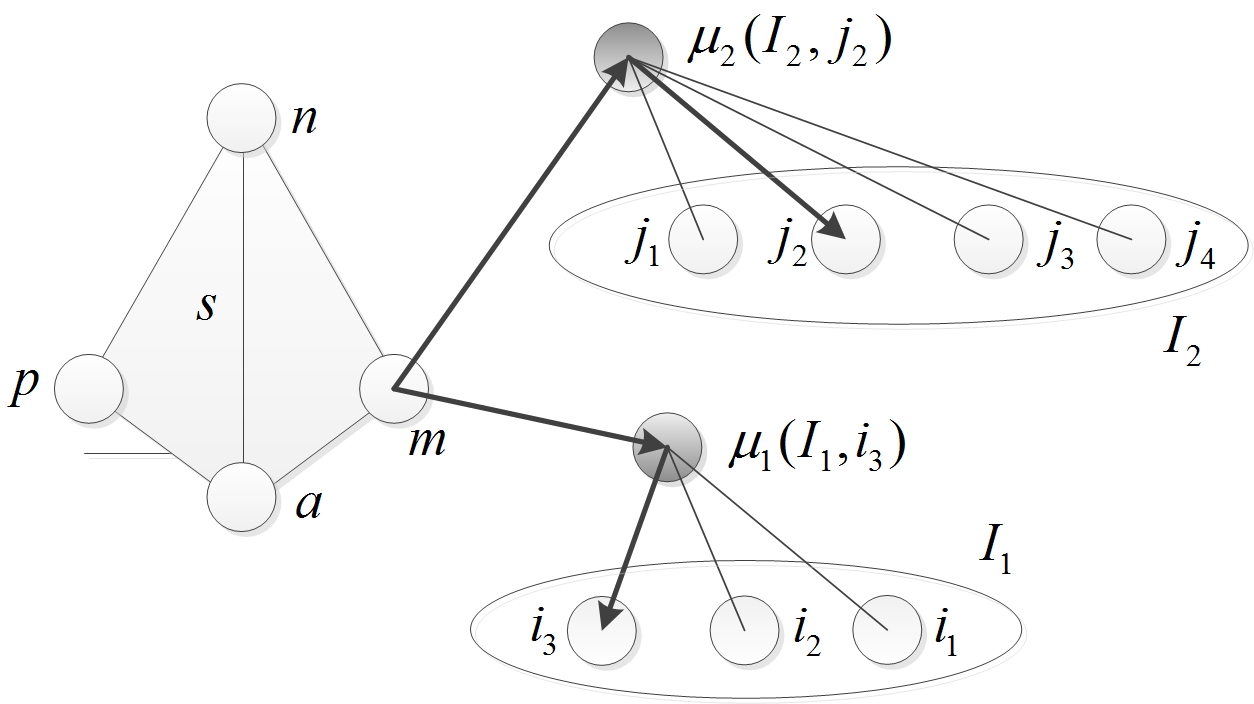
\includegraphics[width=0.7\linewidth]{mean_scene.jpg}
	\caption{Пример структуры значения $m$ знака $s$, которое включает в себя два экземпляра $\mu_1(I_1, i_3)$ и $\mu_2(I_2, j_2)$, где $I_1=\{i_1,i_2,i_3\}$ и $I_2=\{j_1,j_2,j_3,j_4\}$ "--- наборы семантических валентностей.}
	\label{fg:mean_scene}
\end{figure}

Рассмотрим знаки $s_1$ и $s_2$; $\mu_1(I_1,i)$ и $\mu_2(I_2,j)$ "--- экземпляры значений $s_1$ и $s_2$ соответственно. Введём оператор $Des$, который для всякого знака $s_1$ просматривает все остальные знаки и пополняет указанные ниже отношения по следующим правилам.
\begin{enumerate}
	\renewcommand\labelenumi{\theenumi.}
	\item Если $I_1=I_2$ и $i=j$, то $R_1^\prime:=R_2^\prime\cup\{(\mu_1,\mu_2)\}$, $R_2^\prime\subseteq M\times M$.
	\item Если для экземпляра значения $\mu_1$ знака $s_1$ существует экземпляр значения $\mu_2$ знака $s_2$ такое, что $I_1\cap I_2\not =\varnothing$, $I_1\not =I_2$ и $i=j$, то $R_2^\prime:=R_2^\prime\cup\{(\mu_1,\mu_2)\}$, $R_2^\prime\subseteq M\times M$.
	\item Если для экземпляра значения $\mu_1$ знака $s_1$ существует экземпляр значения $\mu_2$ знака $s_2$ такое, что $I_1=I_2$, и $i\not =j$, то $R_6:=R_6\cup\{(\mu_1,\mu_2)\}$, $R_6\subseteq M\times M$ "--- ситуационное отношение.
\end{enumerate}
Аналогично отношениям $R_1$ и $R_3$, отношения $R_1^\prime$ и $R_3^\prime$ являются соответственно отношениями эквивалентности и сходства на множестве значений. 

С каждым экземпляром значения $\mu$ свяжем теперь метку $\tau$, и будем записывать $\mu_1(\tau_1,I_1,i)$ и $\mu_2(\tau_2,I_2,j)$. На множестве меток вводится линейный порядок: для $\forall\tau_1,\tau_2$ справедливо $\tau_1\leqslant\tau_2$ либо $\tau_1\geqslant\tau_2$. Рассмотрим некоторое отношение на $M\times M$. Ограничение этого отношения на $M_{scen}\times M_{scen}$, где $M_{scen}\subseteq M$, будем называть сценарным отношением $R_7$, если оно строится следующим образом.
\begin{enumerate}
	\setcounter{enumi}{3}
	\renewcommand\labelenumi{\theenumi.}
	\item Если $\mu_1\in M_{scen}$, $\mu_2\in M_{scen}$, $I_1\not =I_2$, $i\not =j$ и $\tau_1<\tau_2$, то $R_7:=R_7\cup\{(\mu_1,\mu_2)\}$.
\end{enumerate}	

Элементарным сценарием, порождённым знаком $s$, будем называть множество экземпляров значений $M_{est}(s)$ такое, что для $\forall\mu_1\in M_{est}(s)$ и $\mu_2\in M_{est}(s)$ имеет место:
\begin{itemize}
	\item если $\mu_1\in m$, $\mu_2\in m$ и $\tau_1\geqslant\tau_2$, то $(\mu_1,\mu_2)\in R_7$ (в этом случае сценарное отношение $R_7$ определено на множестве экземпляров значения знака $s$, т.е. $M_{scen}=m$);
	\item если $\mu_1\in m$ и $\mu_2\not\in m$ и $\tau_1\geqslant\tau_2$, то $(\mu_1,\mu_2)\in R_6$.
\end{itemize}

На рис. \ref{fg:mean_relat} приведён пример элементарного сценария $M_{est}(s1)$, порождённого знаком $s_1$, а именно сформированного двумя экземплярами $\mu_2$ и $\mu_3$ значения знака $s_1$ такими, что $(\mu_2,\mu_3)\in R_7$. В примере на рис. \ref{fg:mean_relat} в $M_{est}(s1)$ входят и экземпляры значений $\mu_1$ и $\mu_4$ такие, что $\{(\mu_1,\mu_2),(\mu_3,\mu_4)\}\subseteq R_6$, где $\mu_1$ и $\mu_4$ суть экземпляры значений знаков $s_2$ и $s_3$ соответственно.

\begin{figure}[h]
	\centering
	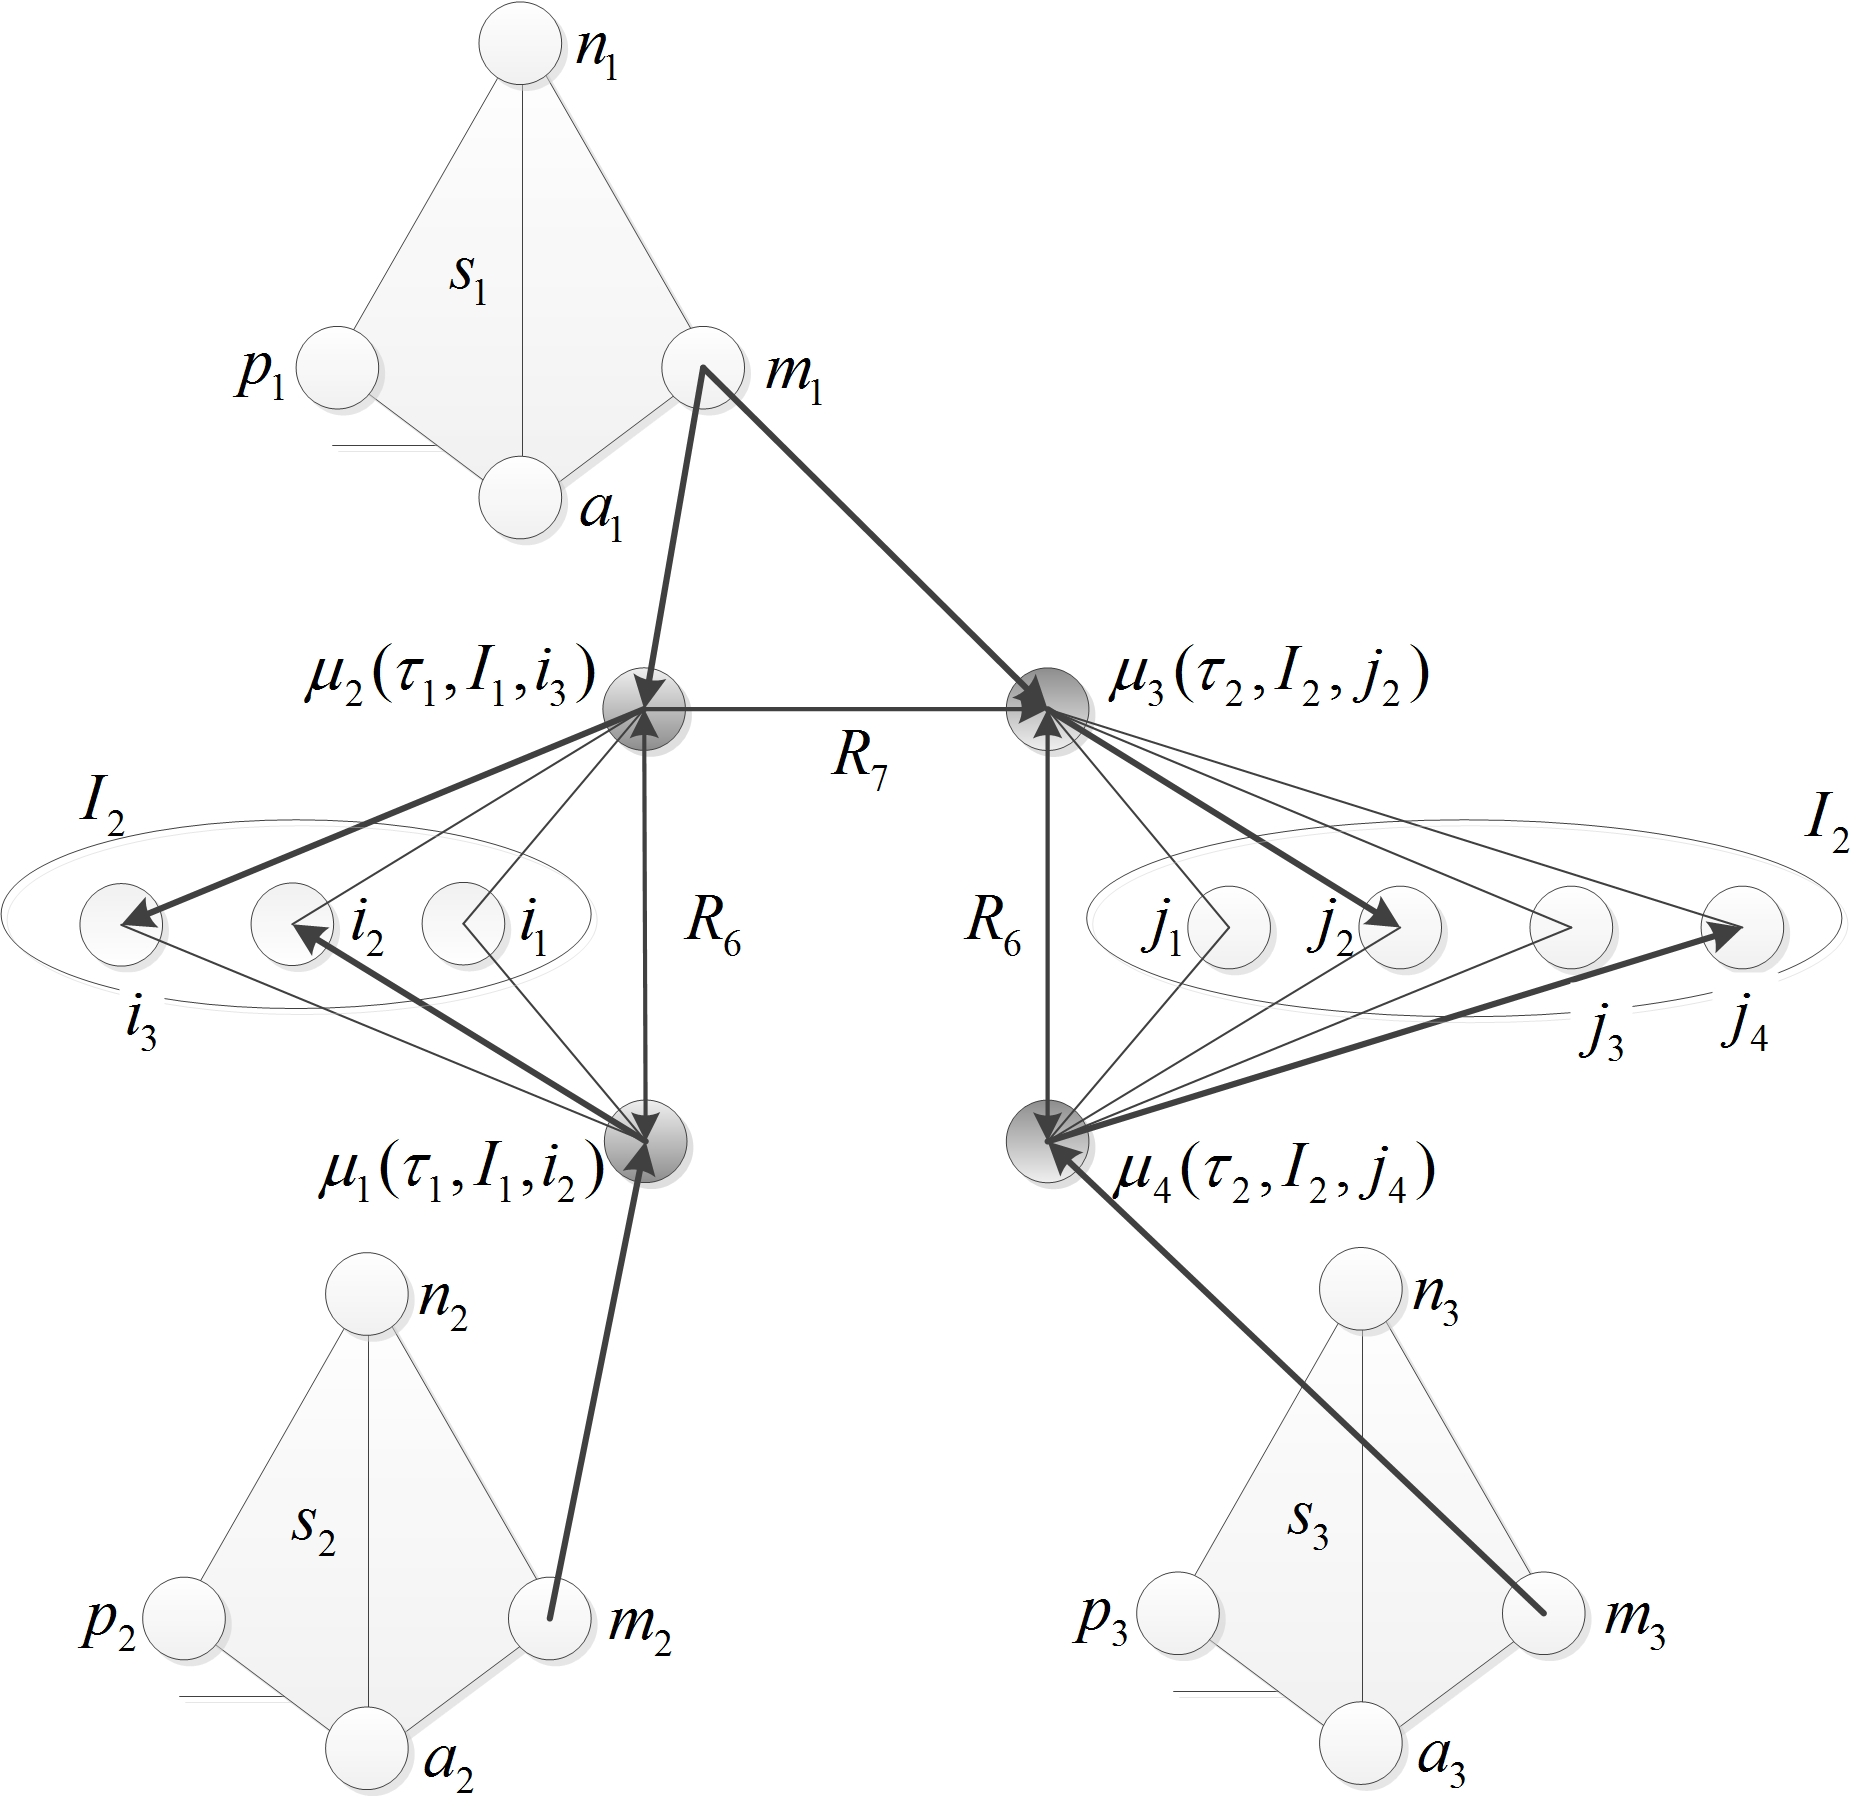
\includegraphics[width=0.7\linewidth]{mean_relat.jpg}
	\caption{Пример элементарного сценария $M_{est}(s_1)=\{\mu_1,\mu_2,\mu_3,\mu_4\}$, порождённого значениями знака $s_1$. Так как в приведённом примере пары экземпляров значений $(\mu_1,\mu_2)$ и $(\mu_3,\mu_4)$ принадлежат отношению $R_6$, а пара $(\mu_1,\mu_3)$ "--- отношению $R_7$, то по определению эти экземпляры принадлежат элементарному сценарию $M_{est}(s_1)$.}
	\label{fg:mean_relat}
\end{figure}

%\newpage
%============================================================================================================================

\clearpage